\documentclass[aspectratio=169]{beamer}

\setbeamersize{text margin left=5mm, text margin right=5mm}

\defbeamertemplate{headline}{my header}{%
\vskip1pt%
\makebox[0pt][l]{\,\insertshortauthor}%
\hspace*{\fill}\insertshorttitle/\insertshortsubtitle\hspace*{\fill}%
\llap{\insertpagenumber/\insertpresentationendpage\,}
}
\setbeamertemplate{headline}[my header]

\let\olditem\item
\renewcommand{\item}{\setlength{\itemsep}{\fill}\olditem}

\usepackage{caption}
\usepackage{soul}
\usepackage{tkz-euclide}
\usetikzlibrary{calc}
\usepackage[]{algorithm2e}
\usepackage{changepage}
\usepackage{amssymb}
\usepackage{xcolor}
\usepackage{mathtools}
\usepackage{tcolorbox}
\usepackage{tikz}
\usepackage{tikz-3dplot}
\usetikzlibrary{arrows.meta, decorations.pathreplacing, positioning, shapes.geometric}

%% Fonts
\usefonttheme{professionalfonts}
\usefonttheme{serif}

\DeclareCaptionLabelFormat{blank}{}
\captionsetup[figure]{labelformat=blank}

%% Math definitions
\def\mf{\ensuremath\mathbf}
\def\mb{\ensuremath\mathbb}
\def\lp{\ensuremath\left(}
\def\rp{\ensuremath\right)}
\def\lv{\ensuremath\left\lvert}
\def\rv{\ensuremath\right\rvert}
\def\lV{\ensuremath\left\lVert}
\def\rV{\ensuremath\right\rVert}
\def\lc{\ensuremath\left\{}
\def\rc{\ensuremath\right\}}
\def\ls{\ensuremath\left[}
\def\rs{\ensuremath\right]}
\def\bmx{\ensuremath\begin{bmatrix*}[r]}
\def\emx{\ensuremath\end{bmatrix*}}
\def\bmxc{\ensuremath\begin{bmatrix*}[c]}
\def\t{\lp t\rp}
\def\k{\ls k\rs}

\newcommand{\demoex}[2]{\onslide<#1->\begin{color}{black!60} #2 \end{color}}
\newcommand{\demoexc}[3]{\onslide<#1->\begin{color}{#2} #3 \end{color}}
\newcommand{\anim}[3]{\onslide<#1->{\begin{color}{#2!60} #3 \end{color}}}
\newcommand{\ct}[1]{\lp #1\rp}
\newcommand{\dt}[1]{\ls #1\rs}
\newcommand{\cols}[2]{\begin{columns}[#1] #2 \end{columns}}
\newcommand{\col}[2]{\begin{column}{#1} #2 \end{column}}

%% Mycolors
\definecolor{myred}{RGB}{192,0,0}
\definecolor{mygray}{RGB}{100,100,100}

%% Custom beamer color
\setbeamercolor{title}{fg=myred}
\setbeamercolor{subtitle}{fg=myred}
\setbeamerfont{title}{series=\bfseries}
% \setbeamercolor{frametitle}{bg=myred, fg=white}
\setbeamercolor{frametitle}{bg=mygray!10!, fg=myred}
\setbeamerfont{frametitle}{series=\bfseries}
\setbeamercolor{item}{fg=mygray}
\setbeamercolor{title in head/foot}{fg=myred}

% Move header to footer
\setbeamertemplate{headline}{}
\setbeamertemplate{footline}{
  \begin{beamercolorbox}[wd=\paperwidth,ht=2.25ex,dp=1ex,center]{footline}
    \inserttitle\hfill\insertauthor\hfill\insertdate\hfill\insertframenumber{}
  \end{beamercolorbox}
}

\title{Applied Linear Algebra in Data Analysis}

% A subtitle is optional and this may be deleted
\subtitle{Solution to Linear Equations}

\author{Sivakumar Balasubramanian}
% - Give the names in the same order as the appear in the paper.
% - Use the \inst{?} command only if the authors have different
%   affiliation.

\institute[Christian Medical College] % (optional, but mostly needed)
{
  \inst{}%
  Department of Bioengineering\\
  Christian Medical College, Bagayam\\
  Vellore 632002
}
% - Use the \inst command only if there are several affiliations.
% - Keep it simple, no one is interested in your street address.

\date{}
% - Either use conference name or its abbreviation.
% - Not really informative to the audience, more for people (including
%   yourself) who are reading the slides online

\subject{Lecture notes on ALADA}
% This is only inserted into the PDF information catalog. Can be left
% out. 

% If you have a file called "university-logo-filename.xxx", where xxx
% is a graphic format that can be processed by latex or pdflatex,
% resp., then you can add a logo as follows:

% \pgfdeclareimage[height=0.5cm]{university-logo}{university-logo-filename}
% \logo{\pgfuseimage{university-logo}}

% Delete this, if you do not want the table of contents to pop up at
% the beginning of each subsection:
\AtBeginSubsection[]
{
  \begin{frame}<beamer>{Outline}
    \tableofcontents[currentsection,currentsubsection]
  \end{frame}
}

% Let's get started
\begin{document}

\begin{frame}
  \titlepage
\end{frame}

% \begin{frame}[t]{References}
% \begin{itemize}
% \item S Boyd, Applied Linear Algebra: Chapters 6, 7, 8, 10 and 11.
% \item G Strang, Linear Algebra: Chapters 1 and 2.
% \end{itemize}
% \end{frame}

\begin{frame}[t]{Linear equations}
\begin{itemize}
\item Matrices present a compact way to represent a set of linear equations. Consider the following,
\[
\begin{rcases*}
\begin{split}
a_{11}x_1 + a_{12}x_2 \ldots + a_{1m}x_m & = b_1 \\
a_{21}x_1 + a_{22}x_2 \ldots + a_{2m}x_m & = b_2 \\
a_{31}x_1 + a_{32}x_2 \ldots + a_{3m}x_m & = b_3 \\
\vdots \\
a_{n1}x_1 + a_{n2}x_2 \ldots + a_{nm}x_m & = b_n \\
\end{split}
\end{rcases*} \, \longrightarrow \mf{Ax} = \mf{b}, \,\,\, \mf{A} \in \mathbb{R}^{n \times m}, \,\, \mf{x} \in \mathbb{R}^m, \,\, \mf{b} \in \mathbb{R}^n
\]

\[
\mf{A} = \begin{bmatrix}
a_{11} & a_{12} & a_{13} & \ldots & a_{1m}\\
a_{21} & a_{22} & a_{23} & \ldots & a_{2m}\\
\vdots & \vdots & \vdots & \ddots & \vdots\\
a_{n1} & a_{n2} & a_{n3} & \ldots & a_{nm}\\
\end{bmatrix} \,\,\,\,\, 
\mf{x} = \begin{bmatrix}
x_1\\ x_2\\ \vdots \\ x_m
\end{bmatrix} \,\,\,\,\,
\mf{b} = \begin{bmatrix}
b_1\\ b_2\\ \vdots \\ b_n
\end{bmatrix}
\]
\end{itemize}
\end{frame}


\begin{frame}[t]{Linear equations in control problems}
\begin{LARGE}
\[ \mf{x}: \text{Input} \,\,\, \mf{b}: \text{Output} \,\,\, \mf{A}: \text{System dynamics} \]

\[ \begin{bmatrix}
b_1\\ b_2\\ \vdots \\ b_n
\end{bmatrix} = \begin{bmatrix}
a_{11} & a_{12} & a_{13} & \ldots & a_{1m}\\
a_{21} & a_{22} & a_{23} & \ldots & a_{2m}\\
\vdots & \vdots & \vdots & \ddots & \vdots\\
a_{n1} & a_{n2} & a_{n3} & \ldots & a_{nm}\\
\end{bmatrix} \,\, \begin{bmatrix}
x_1\\ x_2\\ \vdots \\ x_m
\end{bmatrix} \]
\end{LARGE}
\end{frame}


\begin{frame}[t]{Linear equations in estimation problems}
\begin{LARGE}
\[ \mf{x}: \text{Parameter} \,\,\, \mf{b}: \text{Measurements} \,\,\, \mf{A}: \text{System characteristics} \]

\[ \begin{bmatrix}
b_1\\ b_2\\ \vdots \\ b_n
\end{bmatrix} = \begin{bmatrix}
a_{11} & a_{12} & a_{13} & \ldots & a_{1m}\\
a_{21} & a_{22} & a_{23} & \ldots & a_{2m}\\
\vdots & \vdots & \vdots & \ddots & \vdots\\
a_{n1} & a_{n2} & a_{n3} & \ldots & a_{nm}\\
\end{bmatrix} \,\, \begin{bmatrix}
x_1\\ x_2\\ \vdots \\ x_m
\end{bmatrix} \]
\end{LARGE}
\end{frame}


\begin{frame}[t]{Geometry of linear equations}
\vspace{-0.5cm}
\[\begin{rcases*}
\begin{split} x_1 + 2x_2 &= -1 \\ x_1 + x_2 &= 1 \end{split}
\end{rcases*} \longrightarrow \bmx
1 & 2\\
1 & 1
\emx \bmx
x_1\\
x_2
\emx = \bmx
-1\\
1
\emx\]
Two ways to view this: \textbf{row view} and the \textbf{column view}.
\begin{center}
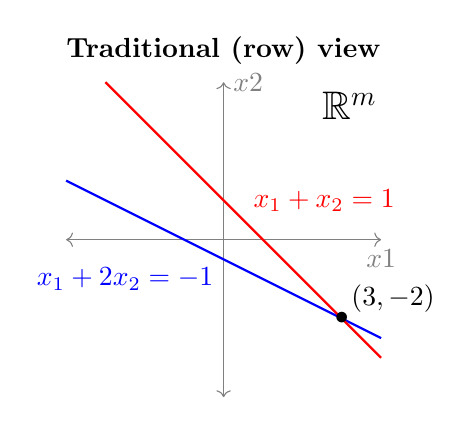
\begin{tikzpicture}[scale=0.5]
\node(0, 0) [yshift=2.4cm] {\textbf{Traditional (row) view}};
\node(0, 0) [xshift=1.6cm,yshift=1.7cm] {\Large {$\mb{R}^m$}};
\draw[gray,<->] (-4, 0) -- (4, 0) node[right,below] {$x1$};
\draw[gray,<->] (0, -4) -- (0, 4) node[right] {$x2$};
\draw[blue,thick] (-4,3/2) -- (4, -5/2) node[midway,left,yshift=-0.25cm] {$x_1 + 2x_2 = -1$};
\draw[red,thick] (-3,4) -- (4, -3) node[midway,right,yshift=0.25cm] {$x_1 + x_2 = 1$};
\draw (3,-2) node[] {$\bullet$};
\draw (3,-2) node[right,yshift=0.25cm] {$\left(3,-2\right)$};
\end{tikzpicture}\hspace{1cm}
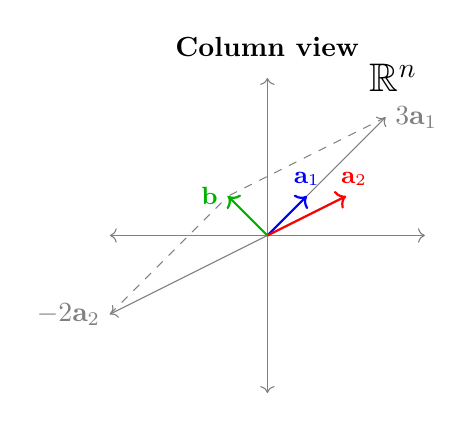
\begin{tikzpicture}[scale=0.5]
\node(0, 0) [yshift=2.4cm] {\textbf{Column view}};
\node(0, 0) [xshift=1.6cm,yshift=2.0cm] {\Large {$\mb{R}^n$}};
\draw[gray,<->] (-4, 0) -- (4, 0);
\draw[gray,<->] (0, -4) -- (0, 4);
\draw[gray,thin,->] (0,0) -- (3,3) node[above,right] {$3\mf{a}_1$};
\draw[blue,thick,->] (0,0) -- (1,1) node[above,yshift=0.cm] {\small{$\mf{a}_1$}};
\draw[red,thick,->] (0,0) -- (2,1) node[above,xshift=0.1cm,yshift=0.cm] {\small{$\mf{a}_2$}};
\draw[gray,thin,->] (0,0) -- (-4,-2) node[below,left] {$-2\mf{a}_2$};
\draw[gray,thin,dashed] (3,3) -- (-1,1);
\draw[gray,thin,dashed] (-4,-2) -- (-1,1);
\draw[black!30!green,thick,->] (0,0) -- (-1,1) node[above,left] {\small{$\mf{b}$}};
\end{tikzpicture}
\end{center}
\end{frame}

\begin{frame}[t]{Solutions of linear equations}
\vspace{-0.5cm}
$$ \mf{Ax = b}, \,\,\, \mf{A} \in \mathbb{R}^{m \times n}, \,\, \mf{x} \in \mathbb{R}^n, \,\, \mf{b} \in \mathbb{R}^m$$
\vspace{-0.5cm}
\begin{itemize}
\item \textbf{Three possible situations:} \textsc{No solution}, \textsc{Infinitely many solutions}, or \textsc{Unique Solution}.
\item When do we have infinitely many or no solutions? In $\mathbb{R}^3$, we can visualize the different situations.
\end{itemize}
\begin{center}
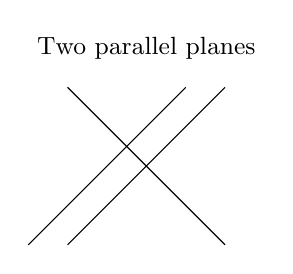
\begin{tikzpicture}[scale=0.5]
\node[yshift=1.5cm] {\small{Two parallel planes}};
\draw[black,-] (-2, -2) -- (2, 2);
\draw[black,-] (-3, -2) -- (1, 2);
\draw[black,-] (2, -2) -- (-2, 2);
\end{tikzpicture}\hspace{0.25cm}
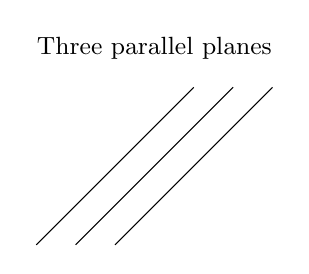
\begin{tikzpicture}[scale=0.5]
\node[yshift=1.5cm] {\small{Three parallel planes}};
\draw[black,-] (-2, -2) -- (2, 2);
\draw[black,-] (-3, -2) -- (1, 2);
\draw[black,-] (-1, -2) -- (3, 2);
\end{tikzpicture}\hspace{0.25cm}
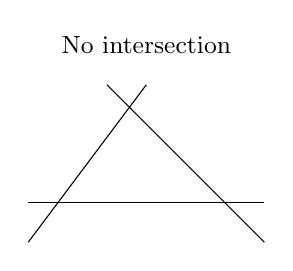
\begin{tikzpicture}[scale=0.5]
\node[yshift=1.0cm] {\small{No intersection}};
\draw[black,-] (-3, -2) -- (3, -2);
\draw[black,-] (-3, -3) -- (0, 1);
\draw[black,-] (3, -3) -- (-1, 1);
\end{tikzpicture}\hspace{0.25cm}
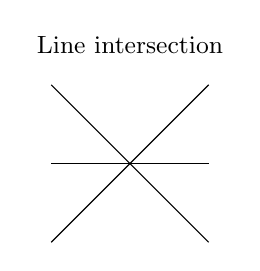
\begin{tikzpicture}[scale=0.5]
\node[yshift=1.5cm] {\small{Line intersection}};
\draw[black,-] (-2, 0) -- (2, 0);
\draw[black,-] (-2, -2) -- (2, 2);
\draw[black,-] (2, -2) -- (-2, 2);
\end{tikzpicture}
\end{center} 
\end{frame}


\begin{frame}[t]{Understanding $\mf{A}\mf{x} = \mf{b}$: Unique solution}

\begin{columns}[t]
\begin{column}{0.3\textwidth}
\[ \bmx
1 & 2\\
1 & 1
\emx\bmx
x_1\\
x_2
\emx = \bmx
-1\\
1
\emx \]
\begin{center}
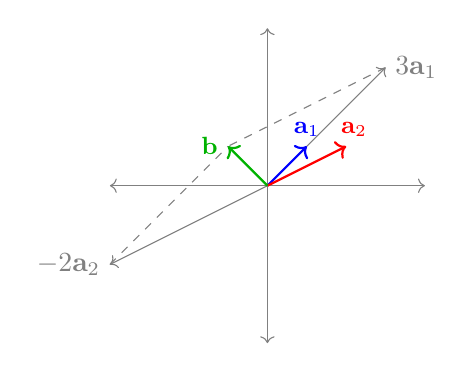
\begin{tikzpicture}[scale=0.5]
\draw[gray,<->] (-4, 0) -- (4, 0);
\draw[gray,<->] (0, -4) -- (0, 4);
\draw[gray,thin,->] (0,0) -- (3,3) node[above,right] {$3\mf{a}_1$};
\draw[blue,thick,->] (0,0) -- (1,1) node[above,yshift=0.cm] {\small{$\mf{a}_1$}};
\draw[red,thick,->] (0,0) -- (2,1) node[above,xshift=0.1cm,yshift=0.cm] {\small{$\mf{a}_2$}};
\draw[gray,thin,->] (0,0) -- (-4,-2) node[below,left] {$-2\mf{a}_2$};
\draw[gray,thin,dashed] (3,3) -- (-1,1);
\draw[gray,thin,dashed] (-4,-2) -- (-1,1);
\draw[black!30!green,thick,->] (0,0) -- (-1,1) node[above,left] {\small{$\mf{b}$}};
\end{tikzpicture}
\end{center}
\end{column}
\hspace{0.5cm}
\begin{column}{0.6\textwidth}
\begin{itemize}
  \item Square matrix
  \item Linearly independent set of columns $\lc \mf{a}_1, \mf{a}_2 \rc$
  \item $\mf{b} \in span\lp{\lc \mf{a}_1, \mf{a}_2 \rc}\rp$.
  \item Always solvable, and give an unique solution.
\end{itemize}
\end{column}
\end{columns}
\end{frame}


\begin{frame}[t]{Understanding $\mf{A}\mf{x} = \mf{b}$: Unique solution or No solution}
\begin{columns}[t]
\begin{column}{0.3\textwidth}
\begin{enumerate}
  \item $\bmx 2\\ 1 \emx \bmx x_1 \emx = \mf{b}_1 = \bmx -1\\ 1 \emx$
  \item $\bmx 2\\ 1 \emx \bmx x_1 \emx = \mf{b}_2 = \bmx 3\\ 1.5 \emx$
\end{enumerate}

\begin{center}
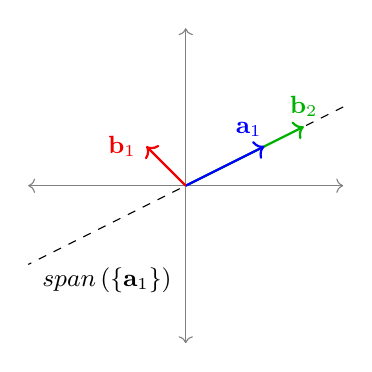
\begin{tikzpicture}[scale=0.5]
\draw[gray,<->] (-4, 0) -- (4, 0);
\draw[gray,<->] (0, -4) -- (0, 4);
\draw[black,dashed] (4, 2) -- (-4,-2) node[xshift=1cm,,yshift=-0.2cm] {\small{$span\lp \lc \mf{a}_1 \rc\rp$}};
\draw[black!30!green,thick,->] (0,0) -- (3,1.5) node[above,xshift=0.0cm,yshift=0.cm] {\small{$\mf{b}_2$}};
\draw[blue,thick,->] (0,0) -- (2,1) node[above,xshift=-0.2cm,yshift=0.cm] {\small{$\mf{a}_1$}};
% \draw[gray,thin,dashed] (3,3) -- (-1,1);
% \draw[gray,thin,dashed] (-4,-2) -- (-1,1);
\draw[black!5!red,thick,->] (0,0) -- (-1,1) node[above,left] {\small{$\mf{b}_1$}};
\end{tikzpicture}
\end{center}
\end{column}
\hspace{0.5cm}
\begin{column}{0.6\textwidth}
\begin{itemize}
  \item Tall matrix
  \item Linearly independent set of columns $\lc \mf{a}_1 \rc$
\end{itemize}
\vspace{0.25cm}
$\mf{b}_1 \notin span\lp{\lc \mf{a}_1 \rc}\rp \implies$ Not solvable.

\vspace{0.25cm}
$\mf{b}_2 \in span\lp{\lc \mf{a}_1 \rc}\rp \implies$ Solvable with unqiue solution.
\end{column}
\end{columns}
\end{frame}


\begin{frame}[t]{Understanding $\mf{A}\mf{x} = \mf{b}$: Infinitely many solution}
\begin{columns}[t]
\begin{column}{0.3\textwidth}
\[ \bmx
1 & 2 & -1\\
1 & 1 & -2
\emx\bmx
x_1\\
x_2\\
x_3
\emx = \bmx
-1\\
1
\emx \]
\begin{center}
\begin{tikzpicture}[scale=0.5]
\draw[gray,<->] (-4, 0) -- (4, 0);
\draw[gray,<->] (0, -4) -- (0, 4);
% \draw[gray,thin,->] (0,0) -- (3,3) node[above,right] {$3a_1$};
\draw[blue,thick,->] (0,0) -- (1,1) node[above,yshift=0.cm] {\small{$\mf{a}_1$}};
\draw[red,thick,->] (0,0) -- (2,1) node[above,xshift=0.1cm,yshift=0.cm] {\small{$\mf{a}_2$}};
\draw[black!30!green,thick,->] (0,0) -- (-1,-2) node[above,xshift=0cm,yshift=-0.4cm] {\small{$\mf{a}_3$}};
\draw[black,thick,->] (0,0) -- (-1,1) node[above,left] {\small{$b$}};
\end{tikzpicture}
\end{center}
\end{column}
\hspace{0.5cm}
\begin{column}{0.6\textwidth}
\begin{itemize}
  \item Fat matrix
  \item Linearly dependent set of columns $\lc \mf{a}_1, \mf{a}_2, \mf{a}_3 \rc$
  \item $\mf{b} \in span\lp{\lc \mf{a}_1, \mf{a}_2, \mf{a}_3 \rc}\rp$.
  \item Always solvable, with infinitely many solutions.
\end{itemize}
\end{column}
\end{columns}
\end{frame}


\begin{frame}[t]{Understanding $\mf{A}\mf{x} = \mf{b}$: Conditions for different types of solutions}
\[ \mf{A}\mf{x} = \mf{b}, \,\,\, \mf{A} \in \mb{R}^{n \times m}, \, \mf{x} \in \mb{R}^m, \, \mf{b} \in \mb{R}^n \]

\textbf{Full rank } $\mf{A}$:
\begin{itemize}
  \item $rank\lp \mf{A} \rp = n \implies$ \textbf{Always solvable}\\
        \vspace{0.2cm}
        $\begin{cases} 
        n = m & \implies \text{Unique solution} \\ 
        n < m & \implies \text{Infinitely many solutions} \\ 
        \end{cases}$
  \item $rank\lp \mf{A} \rp = m  \implies$ \textbf{No infinite solutions}\\
        \vspace{0.2cm}
        $\begin{cases} 
        m = n & \implies \text{Unique solution} \\ 
        m < n & \rightarrow \begin{cases}
        \mf{b} \in span\lp \mf{a}_1, \ldots \mf{a}_m \rp {\implies} \text{Unique solution} \\
        \mf{b} \notin span\lp \mf{a}_1, \ldots \mf{a}_m \rp {\implies} \text{No solution}
        \end{cases}\\ 
        \end{cases}$
\end{itemize}
\end{frame}


\begin{frame}[t]{Understanding $\mf{A}\mf{x} = \mf{b}$: Conditions for different types of solutions}
\[ \mf{A}\mf{x} = \mf{b}, \,\,\, \mf{A} \in \mb{R}^{n \times m}, \, \mf{x} \in \mb{R}^m, \, \mf{b} \in \mb{R}^n \]

\textbf{Rank deficient} $\mf{A}$:
\begin{itemize}
  \item $rank\lp \mf{A} \rp < \min \lp n, m \rp \implies$ \textbf{No unique solution}\\
        \vspace{0.2cm}
        $\begin{cases}
        \mf{b} \in span\lp \mf{a}_1, \ldots \mf{a}_m \rp {\implies} \text{Infinitely many solutions} \\
        \mf{b} \notin span\lp \mf{a}_1, \ldots \mf{a}_m \rp {\implies} \text{No solution}
        \end{cases}$
\end{itemize}
\end{frame}


\begin{frame}[t]{Understanding $\mf{A}\mf{x} = \mf{b}$: Conditions for different types of solutions}
\[ \mf{A}\mf{x} = \mf{b}, \,\,\, \mf{A} \in \mb{R}^{n \times m}, \, \mf{x} \in \mb{R}^m, \, \mf{b} \in \mb{R}^n \]
\vspace{0.5cm}
\begin{itemize}
  \item $\mf{b} \notin span\lp \mf{a}_1, \ldots \mf{a}_m \rp {\implies} \text{No solution}$
  \vspace{-2cm}
  \item $\mf{b} \in span\lp \mf{a}_1, \ldots \mf{a}_m \rp {\implies} \begin{cases}
        rank\lp \mf{A} \rp = m \implies \text{Unique} \\
        rank\lp \mf{A} \rp < m \implies \text{Infinitely many solutions}
        \end{cases}$
\end{itemize}
\end{frame}

\begin{frame}[t]{General solution of linear equations}
\[ \mf{A}\mf{x} = \mf{b}, \,\,\, \mf{A} \in \mb{R}^{n \times m}, \, \mf{x} \in \mb{R}^m, \, \mf{b} \in \mb{R}^n \]

\begin{itemize}
  \item Assuming that this system can be solved, the most general form of the solution is,
  \[ \mf{x} = \mf{x}_p + \mf{x}_h \]
  where, $\mf{x}_p$ is called the particular solution, and $\mf{x}_h$ is the homogenous solution.

  \item \textbf{Homogenous solution}: Solution of the equation $\mf{A}\mf{x} = \mf{0}$.

  \item The set of all homogenous solutions of $\mf{A}$ -- $\lc \mf{x}_h \, \vert \, \mf{A}\mf{x}_h = \mf{0} \rc$ -- form a subspace of $\mb{R}^m$.
\end{itemize}
\end{frame}

\begin{frame}[t]{Geometry of the general solution}
\[ \mf{A}\mf{x} = \mf{b}, \,\,\, \mf{A} \in \mb{R}^{n \times m}, \, \mf{x} \in \mb{R}^m, \, \mf{b} \in \mb{R}^n \]
\begin{columns}[t]
\begin{column}{0.3\textwidth}
\[ \mf{A} = \bmx
1 & -1\\
2 & -2
\emx, \,\, \mf{b} = \bmx
1.5\\
3
\emx \]
\end{column}
\hspace{0.5cm}
\begin{column}{0.6\textwidth}
\end{column}
\end{columns}
\end{frame}

\begin{frame}[t]{Geometry of the general solution}
\begin{center}
\vspace{-0.2cm}
\begin{small}
$\mf{A} = \bmx
1 &  2\\
1 &  1
\emx, \,\, \mf{b} = \bmx
-1\\
1
\emx$
\end{small}
\vspace{0.5cm}

\begin{tikzpicture}[scale=0.45]
\node[] at (-5, 5) {\Large $\mb{R}^m$};
\draw[gray,<->] (-6, 0) -- (6, 0) node[right,below] {$x_1$};
\draw[gray,<->] (0, -6) -- (0, 6) node[right] {$x_2$};
\draw[black,thick,->] (0,0) -- (3,-2);
\node[above] at (3, -2) {$\mf{x}_p$};
\node[black!30!green,above left] at (0, 0) {\small $\mf{x}_h = \mf{0}$};

\node[] at (-5 + 14, 5) {\Large $\mb{R}^n$};
\draw[gray,<->] (-6 + 14, 0) -- (6 + 14, 0);
\draw[gray,<->] (0 + 14, -6) -- (0 + 14, 6);
% \node[above, xshift=-0.5cm]  at (-3.2 + 14, -4) {\small $span\lp \lc \mf{a}_1, \mf{a}_2 \rc \rp$};
% \draw[black!30!green,thick,->] (0 + 14,0) -- (2 + 14,4) node[above,right] {$\mf{b}$};
\draw[red,thick,->] (0 + 14,0) -- (1 + 14,1) node[xshift=-0.1cm,above] {\small $\mf{a}_1$};
\draw[blue,thick,->] (0 + 14,0) -- (2 + 14,1) node[below,yshift=-0.05cm] {\small{$\mf{a}_2$}};
\draw[red,thin,dashed] (-6 + 14,-6) -- (6 + 14,6);
\node[red, rotate=45] at (3 + 14, 3.9) {\small $span\lp\lc \mf{a}_1 \rc\rp$};
\draw[blue,thin,dashed] (-6 + 14,-3) -- (6 + 14,3);
\node[blue, rotate=26.6] at (4.5 + 14, 1.6) {\small $span\lp\lc \mf{a}_2 \rc\rp$};
\draw[black!30!green,thick,->] (0 + 14,0) -- (-1 + 14,1);
\node[above left] at (-1, 1) {\small $\mf{b}$};
\draw[red, thin, -latex] (3+0.1, -2) to[out=30,in=-135] (-1 + 14 - 0.1, 1);
\node[] at (7, -1.5) {$\mf{A}$};
\end{tikzpicture}
\end{center}
\end{frame}


\begin{frame}[t]{Geometry of the general solution}
\begin{center}
\vspace{-0.2cm}
\begin{small}
$\mf{A} = \bmx
2\\
1
\emx, \,\, \mf{b} = \bmx
-4\\
-2
\emx$
\end{small}
\vspace{0.5cm}

\begin{tikzpicture}[scale=0.45]
\node[] at (-5, 5) {\Large $\mb{R}^m$};
\draw[gray,<->] (-6, 0) -- (6, 0) node[right,below] {$x_1$};
\draw[black,thick,->] (0,0) -- (-2,0);
\node[above left] at (-2, 0) {$\mf{x}_p$};
\node[black!30!green,below] at (0, 0) {\small $\mf{x}_h = \mf{0}$};

\node[] at (-5 + 14, 5) {\Large $\mb{R}^n$};
\draw[gray,<->] (-6 + 14, 0) -- (6 + 14, 0);
\draw[gray,<->] (0 + 14, -6) -- (0 + 14, 6);
\draw[blue,thick,->] (0 + 14,0) -- (2 + 14,1) node[below,yshift=-0.05cm] {\small{$\mf{a}_1$}};
\draw[blue,thin,dashed] (-6 + 14,-3) -- (6 + 14,3);
\node[blue, rotate=26.6] at (4.5 + 14, 1.6) {\small $span\lp\lc \mf{a}_1 \rc\rp$};
\draw[black!30!green,thick,->] (0 + 14,0) -- (-4 + 14,-2);
\node[above left] at (-4 + 14, -2) {\small $\mf{b}$};
\draw[red, thin, -latex] (-2, 0 - 0.1) to[out=-90,in=-100] (-4 + 14, -2);
\node[] at (5, -4) {$\mf{A}$};
\end{tikzpicture}
\end{center}
\end{frame}


\begin{frame}[t]{Geometry of the general solution}
\begin{center}
\vspace{-0.2cm}
\begin{small}
$\mf{A} = \bmx
2 &  1
\emx, \,\, \mf{b} = \bmx
5
\emx$
\end{small}
\vspace{0.5cm}


\begin{tikzpicture}[scale=0.45]
\node[] at (-5, 5) {\Large $\mb{R}^m$};
\draw[gray,<->] (-6, 0) -- (6, 0) node[right,below] {$x_1$};
\draw[gray,<->] (0, -6) -- (0, 6) node[right] {$x_2$};
\draw[black,thick,->] (0,0) -- (2,1);
\node[] at (1, 1.2) {$\mf{x}_p$};
\draw[black!30!green,thick,dotted] (-3, 6) -- (3,-6);
\node[black!30!green,below,rotate=-63.43] at (3, -3) {\small $\lc \mf{x}_h \, \vert \, \mf{A}\mf{x}_h = \mf{0} \rc$};
\draw[black!30!green,thick] (5.5,-6) -- (-0.5,6);
\node[black!30!green,rotate=-63.43] at (1.2, 4) {\small $\mf{x}_p + \mf{x}_h$};

\node[] at (5 + 14, 5) {\Large $\mb{R}^n$};
\draw[gray,<->] (-6 + 14, 0) -- (6 + 14, 0);
\draw[black,thick,->] (0 + 14,0) -- (5 + 14,0);
\node[below] at (5 + 14, 0) {\small $\mf{b}$};
% \draw[gray,<->] (0 + 14, -6) -- (0 + 14, 6);
% \draw[black,thick,dashed] (3 + 14,6) -- (-3 + 14,-6);
% \node[above, xshift=-0.5cm]  at (-3.2 + 14, -4) {\small $span\lp \lc \mf{a}_1, \mf{a}_2 \rc \rp$};
% \draw[black!30!green,thick,->] (0 + 14,0) -- (2 + 14,4) node[above,right] {$\mf{b}$};
% \draw[red,thick,->] (0 + 14,0) -- (1 + 14,2) node[above,right] {$\mf{a}_1$};
% \draw[blue,thick,->] (0 + 14,0) -- (-1 + 14,-2) node[above,xshift=-0.25cm] {\small{$\mf{a}_2$}};
\draw[red, thin, -latex] (1.5 + 0.1, 2) to[out=30,in=90] (5 + 14, 0 + 0.1);
\node[] at (9, 5.5) {$\mf{A}$};
\end{tikzpicture}
\end{center}
\end{frame}


\begin{frame}[t]{Geometry of the general solution}
\begin{center}
\vspace{-0.2cm}
\begin{small}
$\mf{A} = \bmx
1 & -1\\
2 & -2
\emx, \,\, \mf{b} = \bmx
2\\
4
\emx$
\end{small}
\vspace{0.5cm}

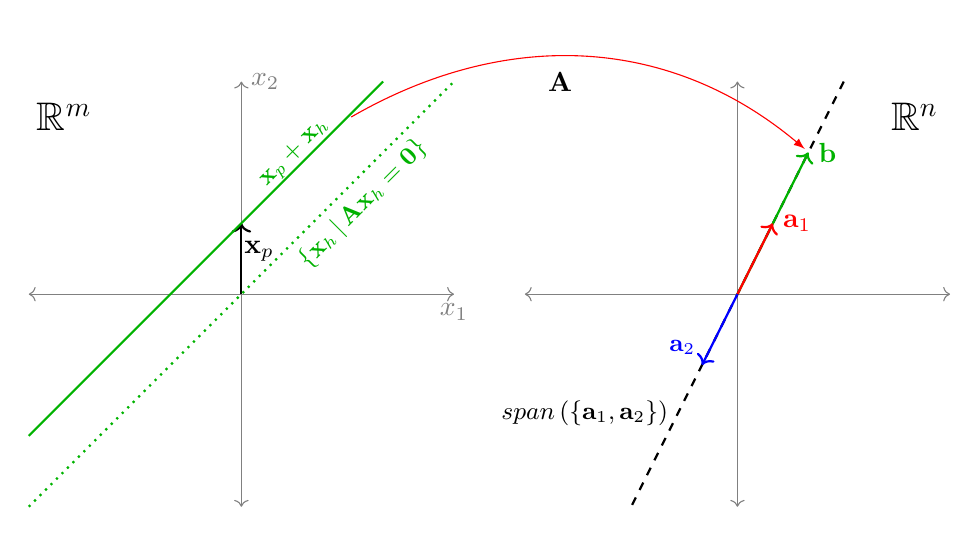
\begin{tikzpicture}[scale=0.45]
\node[] at (-5, 5) {\Large $\mb{R}^m$};
\draw[gray,<->] (-6, 0) -- (6, 0) node[right,below] {$x_1$};
\draw[gray,<->] (0, -6) -- (0, 6) node[right] {$x_2$};
\draw[black,thick,->] (0,0) -- (0,2);
\node[] at (0.5, 1.2) {$\mf{x}_p$};
\draw[black!30!green,thick,dotted] (-6,-6) -- (6,6);
\node[black!30!green,below,rotate=45] at (3, 3) {\small $\lc \mf{x}_h \, \vert \, \mf{A}\mf{x}_h = \mf{0} \rc$};
\draw[black!30!green,thick] (-6,-4) -- (4,6);
\node[black!30!green,rotate=45] at (1.5, 4) {\small $\mf{x}_p + \mf{x}_h$};

\node[] at (5 + 14, 5) {\Large $\mb{R}^n$};
\draw[gray,<->] (-6 + 14, 0) -- (6 + 14, 0);
\draw[gray,<->] (0 + 14, -6) -- (0 + 14, 6);
\draw[black,thick,dashed] (3 + 14,6) -- (-3 + 14,-6);
\node[above, xshift=-0.5cm]  at (-3.2 + 14, -4) {\small $span\lp \lc \mf{a}_1, \mf{a}_2 \rc \rp$};
\draw[black!30!green,thick,->] (0 + 14,0) -- (2 + 14,4) node[above,right] {$\mf{b}$};
\draw[red,thick,->] (0 + 14,0) -- (1 + 14,2) node[above,right] {$\mf{a}_1$};
\draw[blue,thick,->] (0 + 14,0) -- (-1 + 14,-2) node[above,xshift=-0.25cm] {\small{$\mf{a}_2$}};
\draw[red, thin, -latex] (3.1, 5) to[out=30,in=140] (2 + 14 - 0.1, 4 + 0.1);
\node[] at (9, 6) {$\mf{A}$};
\end{tikzpicture}
\end{center}
\end{frame}

\begin{frame}[t]{Four Fundamental Subspaces of $\mf{A} \in \mb{R}^{n \times m}$}
\begin{itemize}
    \item $\mathcal{C}\left(\mf{A}\right)$: \textbf{Column Space of} $\mf{A}$ -- the span of the columns of $\mf{A}$.
    \[ \mathcal{C}\left(\mf{A}\right) = \left\{\mf{Ax} \left|\right. \mf{x} \in \mathbb{R}^m\right\} \subseteq \mathbb{R}^n \]

    \item $\mathcal{N}\left(\mf{A}\right)$: \textbf{Nullspace of} $\mf{A}$ -- the set of all $\mf{x} \in \mathbb{R}^m$ that are mapped to zero by $\mf{A}$.
    \[ \mathcal{N}\left(\mf{A}\right) = \left\{\mf{x} \left|\right. \mf{Ax}  = \mf{0}\right\} \subseteq \mathbb{R}^m \]
    
    \item $\mathcal{C}\left(\mf{A}^{\top}\right)$: \textbf{Row Space of} $\mf{A}$ -- the span of the rows of $\mf{A}$.
    \[ \mathcal{C}\left(\mf{A}^{\top}\right) = \left\{\mf{A}^{\top}\mf{y} \left|\right. \mf{y} \in \mathbb{R}^n\right\} \subseteq \mathbb{R}^m \]

    \item $\mathcal{N}\left(\mf{A}^{\top}\right)$: \textbf{Nullspace of} $\mf{A}^{\top}$ -- the set of all $\mf{y} \in \mathbb{R}^n$ that are mapped to zero by $\mf{A}^{\top}$.
    \[ \mathcal{N}\left(\mf{A}^{\top}\right) = \left\{\mf{y} \left|\right. \mf{A}^{\top}\mf{y}  = \mf{0}\right\} \subseteq \mathbb{R}^n \]

    This is also called the \textbf{left nullspace} of $\mf{A}$.
\end{itemize}
\end{frame}

\begin{frame}[t]{Linear Independence}
\begin{itemize}
    \item Given a set of vectors $\left\{\mf{v}_1, \mf{v}_2, \ldots \mf{v}_m\right\}, \,\,\, \mf{v}_i \in \mathbb{R}^n$, how can we determine if this set is linear independent?
    \item We need to verify, $a_1 \mf{v}_1 + a_2 \mf{v}_2 + \cdots + a_m \mf{v}_m= 0$
    \[ \begin{rcases*}\begin{bmatrix} \mf{v}_1 & \cdots & \mf{v}_m\end{bmatrix} \begin{bmatrix} a_1 \\ \vdots \\ a_m\end{bmatrix} = \begin{bmatrix} 0 \\ \vdots \\ 0\end{bmatrix} = \mf{V}\mf{a} = \mf{0}\end{rcases*} \mathcal{N}\left(\mf{V}\right) = \left\{\mf{0}\right\}, \,\,\, rank\left(\mf{V}\right) = n  \]
    \item This is also equivalent to saying that when the $rank \left(\mf{A}\right) = n \implies$ the columns of $\mf{A}$ form an independent set of vectors.
    \item When do the rows of $\mf{A}$ form an independent set?
    \item What about both rows and columns? When does that happen?
\end{itemize}
\end{frame}


\begin{frame}[t]{Dimension of the four fundamental subspaces}
\begin{itemize}
    \item \textbf{Column space} $C(\mf{A})$
    \begin{itemize}
        \item $\dim \,C(\mf{A}) = rank\left(\mf{A}\right) = r$
    \end{itemize}
    \item \textbf{Nullspace} $N(\mf{A})$
    \begin{itemize}
        \item $\dim \,N(\mf{A}) = n-r$
    \end{itemize}
    \item \textbf{Row space} $C(\mf{A}^{\top})$
    \begin{itemize}
        \item $\dim \,C(\mf{A}^{\top}) = rank\left(\mf{A}^{\top}\right) = rank\left(\mf{A}\right) = r$
    \end{itemize}
    \item \textbf{Left Nullspace} $N(\mf{A}^{\top})$
    \begin{itemize}
        \item $\dim \,N(\mf{A}^{\top}) = m-r$
    \end{itemize}
\end{itemize}
\end{frame}


\end{document}